\documentclass[tikz,border=5pt]{standalone}
\usetikzlibrary{shapes.geometric}
\begin{document}
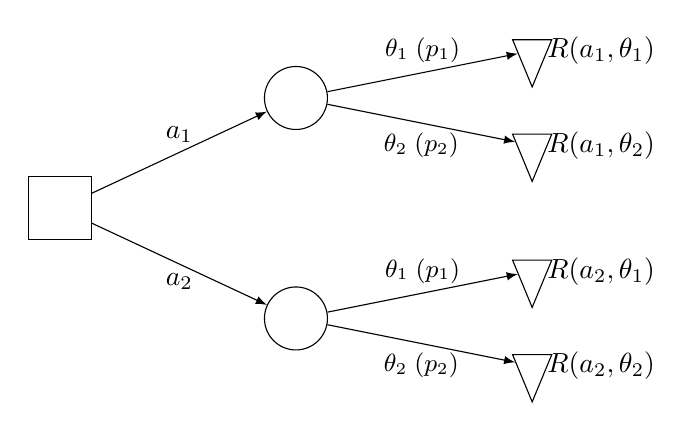
\begin{tikzpicture}[
  grow=right, level distance=3cm, sibling distance=1.2cm,
  decision/.style={rectangle, draw, minimum size=8mm},
  chance/.style={circle, draw, minimum size=8mm},
  terminal/.style={isosceles triangle, draw, shape border rotate=-90, minimum height=6mm, minimum width=4mm},
  edge from parent/.style={draw, -latex},
  level 1/.style={sibling distance=2.8cm},
  level 2/.style={sibling distance=1.2cm}
]
\node [decision] {}
  child {node [chance] {}
    child {node [terminal] {} node[right=2pt] {$R(a_2, \theta_2)$}
      edge from parent node[below] {\small $\theta_2\;(p_2)$}}
    child {node [terminal] {} node[right=2pt] {$R(a_2, \theta_1)$}
      edge from parent node[above] {\small $\theta_1\;(p_1)$}}
    edge from parent node[below] {$a_2$}
  }
  child {node [chance] {}
    child {node [terminal] {} node[right=2pt] {$R(a_1, \theta_2)$}
      edge from parent node[below] {\small $\theta_2\;(p_2)$}}
    child {node [terminal] {} node[right=2pt] {$R(a_1, \theta_1)$}
      edge from parent node[above] {\small $\theta_1\;(p_1)$}}
    edge from parent node[above] {$a_1$}
  };
\end{tikzpicture}
\end{document}
